\documentclass{article}
\usepackage[utf8]{inputenc}
\usepackage{graphicx}
\usepackage[spanish]{babel}

\begin{document}

\begin{figure}[t!]

\includegraphics[scale=0.3]{logo_udp.PNG}
\label{fig:udplogo}
\end{figure}

\title{\textbf{{Scapy y Wireshark \\ Redes de Datos \vspace{10cm}}}}
\author{\hspace{8cm} Vicente Henriquez \\ \hspace{8cm} Franco Montenegro}
\date{\hspace{8cm} 13/09/2017}
\maketitle

\newpage
\tableofcontents
\newpage
\section{Introducción \vspace{0.5cm}}
La creación y envío de paquetes de datos es una parte importante de la comunicación, analizar este proceso es clave para entender que sucede en los distintos casos que puede presentar la transmisión de datos, por lo que nos ayudaremos con dos programas: Scapy y Wireshark, que son un creador de paques y un analizador de trafíco de red respectivamente.

\newpage
\section{Desarrollo \vspace{0.5cm}}
\subsection{Creación de Paquetes \vspace{0.3cm}}
Se nos solicita crear tres paquetes en Scapy de tipo ICMP:
\begin{itemize}
    \item Dirección de MAC de destino FF:FF:FF:FF:FF:FF (Figura \ref{fig:paq1})\\
\begin{figure}[h!]
\centering
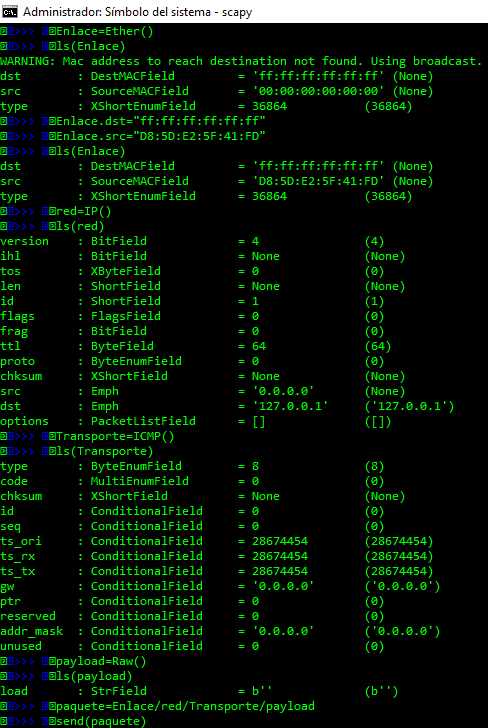
\includegraphics[scale=05, width=12cm, height=14cm]{sshot-1.png}
\caption{Paquete 1}
\label{fig:paq1}
\end{figure}
    
    \item Dirección de MAC de destino de otro equipo de la red (Figura \ref{fig:paq2})\\
\begin{figure}[h!]
\centering
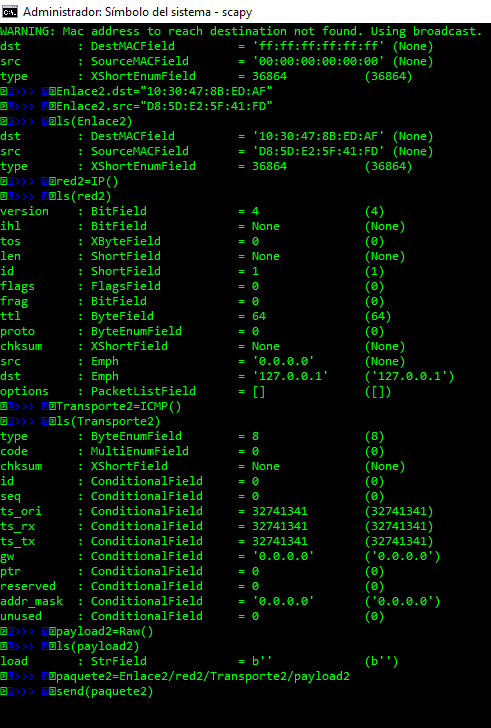
\includegraphics[scale=05, width=12cm, height=14cm]{sshot-2.png}
\caption{Paquete 2}
\label{fig:paq2}
\end{figure}
    \newpage
    \item Dirección de MAC de destino a un equipo que no esté en la red (Figura \ref{fig:paq3}).\\
\begin{figure}[h!]
\centering
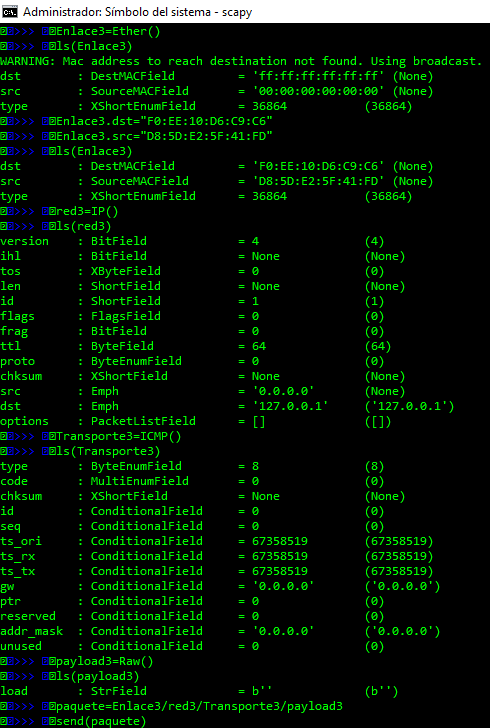
\includegraphics[scale=05, width=12cm, height=14cm]{sshot-3.png}
\caption{Paquete 2}
\label{fig:paq3}
\end{figure}

\end{itemize}

\newpage
\subsection{Analizar la Red \vspace{0.3cm}}
Wireshark es un analizador de protocolos open-source, su principal objetivo es el analizar el tráfico y solucionar problemas de una red además de ser una excelente aplicación didáctica para el estudio de redes.
\begin{itemize}
    \item ¿Qué sucede con una contraseña en una página
HTTPS?\\
\newline Al ser una página https el paquete se encuentra cifrado o encriptado por lo cual no se puede observar los datos que fueron ingresados como en las páginas http, eso si existen diferentes métodos por los cuales uno puede desencriptar el paquete y los datos, los cuales no fueron estudiados.
    \item Identifique las 7 capas del modelo ISO al entrar
a una página.\\
\newline En la Figura \ref{fig:cap1}:
\begin{figure}[h!]
\centering
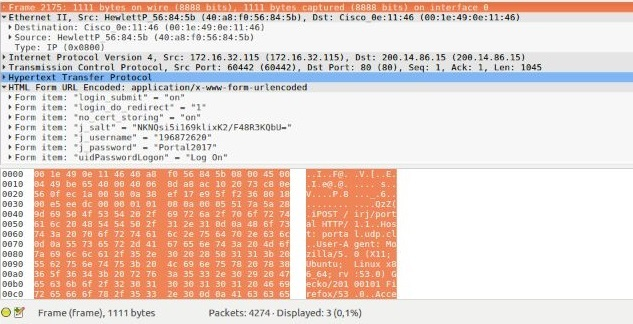
\includegraphics[scale=0.8]{cap.jpg}
\caption{Wireshark}
\label{fig:cap1}
\end{figure}
\begin{enumerate}
    \item Frame se refiere a la capa física.
    \item Ethernet II es capa de enlace.
    \item Internet protocol versión 4 es capa de red.
    \item Transmission control protocol es la capa de transporte.
    \item Hypertext transfer protocol es la capa de sesión.
    \item Html se refiere a la capa de presentación.
    \item La capa de aplicación refiera a la página http.
\end{enumerate}
    \item ¿Qué sucede con la contraseña al entrar a una
página FTP?\\
\newline FTP es un protocolo de transferencia de ficheros entre sistemas conectados a una red, basado en la arquitectura cliente-servidor, de manera que desde un equipo cliente nos podemos conectar a un servidor para descargar ficheros desde el o para enviarle nuestros propios archivos, el servicio es ofrecido por la capa de aplicación del modelo de capas de red TCP/IP, está pensado para ofrecer la máxima velocidad pero en seguridad se queda atrás ya que todo el intercambio de información se realiza en texto plano sin ningún tipo de encriptación o cifrado, por lo cual cualquiera puede interferir y saber los datos de log in en esa página.
\end{itemize}
\subsection{Cuestionario \vspace{0.3cm}}
\begin{enumerate}

\item¿Qué sucede cuando envió un paquete a la dirección FF:FF:FF:FF:FF:FF? ¿Quiénes lo reciben? ¿Por qué?\\
\newline Dicha dirección corresponde a un broadcast, es decir, cuando se envía un paquete con dirección FF:FF:FF:FF:FF:FF le llegará a todos los dispositivos presentes en la red, envío que será limitado por un router.
\item¿Qué pasa cuando envió un paquete con MAC destino a un equipo que no se encuentra en la red? ¿Quiénes lo reciben? ¿Por qué?\\
\newline Luego de verificar que la IP asociada a esa MAC no se encuentra en nuestra red, el ''nuevo'' destinatario será el router, el cual se encargará de encontrar la red que contenga al dispositivo con dicha dirección. Por lo tanto el paquete lo recibe el router de nuestra red, el router de la red receptora y finalmente el equipo que posea la dirección a la que enviamos nuestro paquete.

\item¿Qué pasa cuando envió un paquete con MAC destino a un equipo de la red? ¿Quiénes lo reciben? ¿Por qué?\\
\newline Luego de averiguar la IP que esta asociada a dicha dirección, se puede enviar el paquete directamente desde el emisor al receptor.

\item¿Cuál es la diferencia entre una página HTTP y otra HTTPS?\\
\newline El protocolo HTTP (“Hypertext Transfer Protocol”) es un lenguaje que sirve para intercambiar información entre servidor y cliente, y se diferencia de HTTPS (“Hypertext Transfer Protocol Secure”) porque en HTTPS cualquier dato o información que introduzcas será cifrado, lo que garantiza que no podrá ser vista por nadie más que el cliente y servidor, al contrario HTTP no cifra y cualquiera puede acceder a estos datos.

\item¿En que podría influir en una compañía que los datos no sean seguros? Fundamente su respuesta.\\
\newline Si la compañía no contiene cifrado o su página es HTTP cualquier persona es capaz de entrar en la comunicación servidor-cliente y sacar información o inclusive logearse en tal compañía siendo capaz de hacerse pasar por un trabajador de la compañía, un ejemplo es el mismo portal de la universidad, cualquiera puede saber tu contraseña y asi acceder a tus datos privados, pero a diferencia de una gran compañía no se guardan datos de gran utilidad.

\end{enumerate}
\newpage
\section{Conclusión \vspace{0.5cm}}
La importancia de analizar el proceso de la transmisión de datos queda reflejado en este laboratorio puesto que entender qué es lo que estamos trabajando es vital para saber como manejarlo a futuro ya sea en implementar o arreglar fallos en los envios de paquetes de datos.
\end{document}
